\chapter{الرسل الكيميائية ونقل الإشارة}\label{ch:b2:cell-signalling}

جزيء واحد من الأدرينالين، إذ يصل إلى سطح خلية
كبدية، لا يدخلها قط. بل يرتبط ببروتين على الخارج، فيغير
تشكيل البروتين، وفي غضون ثانية تكون الخلية قد صنعت عشرة
آلاف جزيء من رسول ثانٍ، وفعّلت مئة
ألف جزيء إنزيمي، وبدأت تطلق مليون جزيء
من الغلوكوز --- وهي سلسلة تضخيم طولها مليون ضعف، بدأتها
إشارة بقيت خارج الباب. وهذا الفصل في
الرسل التي ترسلها الخلايا بعضها إلى بعض، وفي كيف تحوّل الخلية
رسالةً على سطحها إلى تغير في كيميائها أو مورّثاتها أو
شكلها: المستقبلات، والرسل الثواني، وشلالات
الكينازات، والتصميمين --- الإشارة السريعة الموصولة بأسلاك في الأعصاب
والإشارة البطيئة المذاعة في الهرمونات --- اللذين يجري تقابلهما
في بقية هذا الكتاب.

\section{الرسل}

\begin{definition}[أصناف الإشارة الكيميائية]\label{def:b2:cell-signalling:kinds}
\index{هرمون}\index{إشارة صماوية}\index{إشارة نظيرة صماوية}\index{ناقل عصبي}
تشير خلية إلى أخرى بجزيء مفروز، هو
\emph{رسول} أو \emph{ربيطة}، يرتبط \emph{بمستقبِل} على
الهدف أو فيه. فبحسب المدى: الإشارة \emph{الصماوية}، ويُطلق فيها
\emph{هرمون} في الدم من غدة فيبلغ
كل خلية في الجسم، ولا يفعل إلا في التي تحمل المستقبل،
على مدى دقائق إلى ساعات (الأنسولين، والكورتيزول، والأدرينالين، والثيروكسين)؛
والإشارة \emph{النظيرة الصماوية}، وينتشر فيها الرسول إلى
الخلايا المجاورة في حدود مليمتر ويُتلَف في الطريق
(عوامل النمو، والهيستامين، والبروستاغلاندينات، ومولدات الشكل في
\cref{ch:b2:vertebrate-development})؛ و\emph{الذاتية}، وفيها تشير الخلية
إلى نفسها؛ و\emph{المشبكية}، ويطلق فيها عصبون
\emph{ناقلًا عصبيًا} عبر فجوة \qty{20}{nm} على
خلية هدف واحدة، في مليثانية (\cref{ch:b2:neurons-synapses}).
وبحسب الكيمياء: الرسل \emph{الذائبة في الماء} --- ومنها مشتقات
الحموض الأمينية كالأدرينالين، والببتيدات والبروتينات كالأنسولين ---
لا تستطيع عبور الغشاء وتفعل في مستقبلات سطحية؛
والرسل \emph{الذائبة في الدسم} --- أي الستيروئيدات (الكورتيزول،
والإستراديول، والتستوستيرون)، والثيروكسين، وحمض الريتينوئيك، وأكسيد النتريك ---
تعبره وتفعل في مستقبلات في الداخل. والجملتان الصماوية والعصبية
هما الطريقان اللذان ينسق بهما جسم من $10^{13}$ خلية
نفسه: فالأولى تذيع ببطء إلى الجميع، والأخرى توصل سلكًا
بسرعة إلى واحد.
\end{definition}

\begin{omfigure}
\begin{tikzpicture}[every node/.style={font=\scriptsize}, >=stealth]
  % endocrine
  \begin{scope}
    \draw[thick, fill=omProp!25] (0,1.6) circle (0.35); \node[above] at (0,2.0) {غدة};
    \draw[very thick, omThm!60] (-0.5,0.6) -- (4.5,0.6); \draw[very thick, omThm!60] (-0.5,0.2) -- (4.5,0.2); \node[omThm!70!black] at (2,0.4) {دم};
    \foreach \x in {0.6,1.5,2.4,3.3} \fill[omProp] (\x,0.4) circle (0.05);
    \draw[->, omProp] (0,1.25) -- (0,0.65);
    \draw[thick, fill=omDef!20] (3.8,-0.8) circle (0.35); \node[below, align=center] at (3.8,-1.2) {خلية هدف\\ذات مستقبل};
    \draw[->, omProp] (3.8,0.15) -- (3.8,-0.4);
    \draw[thick, fill=gray!20] (1.0,-0.8) circle (0.35); \node[below, align=center] at (1.0,-1.2) {بلا مستقبل:\\تتجاهله};
    \node[align=center] at (2.2,-2.4) {صماوية: هرمون في الدم،\\الجسم كله، من دقائق إلى ساعات};
  \end{scope}
  % paracrine
  \begin{scope}[xshift=6.6cm]
    \draw[thick, fill=omProp!25] (0.8,0.6) circle (0.35);
    \foreach \a in {0,45,...,315} \fill[omProp] (0.8,0.6) ++(\a:0.6) circle (0.04);
    \draw[thick, fill=omDef!20] (1.9,0.9) circle (0.3); \draw[thick, fill=omDef!20] (1.7,-0.2) circle (0.3); \draw[thick, fill=omDef!20] (-0.2,0.0) circle (0.3);
    \node[align=center] at (0.8,-2.4) {نظيرة صماوية: ينتشر إلى\\الجيران، ويُتلف\\في حدود مليمتر};
  \end{scope}
  % synaptic
  \begin{scope}[xshift=11.6cm]
    \draw[very thick, omDef] (0,1.8) -- (0,0.5); \draw[thick, fill=omDef!25] (0,0.3) circle (0.25);
    \draw[thick, fill=omExo!30] (0,-0.5) circle (0.3);
    \foreach \x in {-0.08,0,0.08} \fill[omProp] (\x,-0.05) circle (0.03);
    \node[align=center] at (0.2,-2.4) {مشبكية: هدف واحد،\\\qty{20}{nm}،\\مليثانية};
  \end{scope}
\end{tikzpicture}

{\small ثلاثة مديات للإشارة الكيميائية: \omterm{def:b2:cell-signalling:kinds}{هرمون} يذيعه
الدم إلى كل خلية تحمل مستقبله؛ وعامل نظير صماوي
يبلغ جيرانه؛ \omterm{def:b2:cell-signalling:kinds}{وناقل عصبي} يُسلَّم عبر
مشبك إلى خلية واحدة.}
\end{omfigure}

\begin{theorem}[إشغال المستقبلات]\label{thm:b2:cell-signalling:occupancy}
\index{ثابت التفكك}\index{إشغال المستقبلات}
يرتبط المستقبل $R$ بربيطته $L$ ارتباطًا عكوسًا، $R + L
\rightleftharpoons RL$، وله \emph{ثابت تفكك} $K_d =
[R][L]/[RL]$. وعند التوازن يكون كسر المستقبلات المشغولة
\[
\theta = \frac{[RL]}{[R]_{\text{الكلي}}} = \frac{[L]}{K_d + [L]},
\]
وهو القطع الزائد نفسه الذي لإشباع إنزيم. و$K_d$ هو
التركيز الذي يُشغل عنده نصف المستقبلات، وهو مقياس
\emph{الألفة}: فكلما انخفض اشتد الارتباط. ولمستقبلات الهرمونات
$K_d$ في مجال النانومول إلى البيكومول، مطابق
للتراكيز التي تدور بها الهرمونات ($10^{-12}$ إلى
$10^{-9}$ mol/L): فعند $[L] = K_d/10$ يُشغل العُشر، وعند
$10K_d$ تسعة أعشار. ولا تستطيع خلية أن تستجيب \omterm{def:b2:cell-signalling:kinds}{لهرمون} لا
تملك مستقبلات له، وهي تعاير حساسيتها بتغيير
عدد المستقبلات، أو --- كما في \cref{ch:b2:reproductive-hormones}
--- بسحبها حين يكون \omterm{def:b2:cell-signalling:kinds}{الهرمون} حاضرًا على الدوام.
\end{theorem}
\begin{proof}
بوضع $[R] = [R]_{\text{الكلي}} - [RL]$ يكون $K_d = ([R]_{\text{الكلي}} -
[RL])[L]/[RL]$، ومن ثم $[RL](K_d + [L]) = [R]_{\text{الكلي}}[L]$، وهي
الصيغة المطلوبة. وهي عبارة ميكاييليس--منتن في مجلد السنة
الأولى دون الخطوة الحفزية.
\end{proof}

\begin{omfigure}
\begin{tikzpicture}
\begin{axis}[
  width=0.68\linewidth, height=5.2cm,
  axis x line=bottom, axis y line=left,
  xmode=log, xmin=0.01, xmax=100, ymin=0, ymax=1.1,
  xlabel={تركيز الربيطة (بوحدات $K_d$)}, ylabel={كسر المستقبلات المشغولة},
  xlabel style={font=\small, at={(axis description cs:0.5,-0.13)}, anchor=north},
  ylabel style={font=\small},
  tick label style={font=\small}, xtick={0.01,0.1,1,10,100}, ytick={0,0.5,1},
  clip=false,
]
\addplot[very thick, omDef, domain=0.01:100, samples=100] {x/(1+x)};
\draw[dashed, gray] (axis cs:1,0) -- (axis cs:1,0.5) -- (axis cs:0.01,0.5);
\node[font=\scriptsize, anchor=north west] at (axis cs:1.1,0.48) {$[L] = K_d$: نصف الإشغال};
\node[font=\scriptsize, anchor=south east] at (axis cs:0.1,0.1) {10\% عند $K_d/10$};
\node[font=\scriptsize, anchor=north west] at (axis cs:10,0.92) {90\% عند $10\,K_d$};
\end{axis}
\end{tikzpicture}

{\small \omterm{thm:b2:cell-signalling:occupancy}{إشغال المستقبلات} في مقابل تركيز الربيطة على مقياس
لوغاريتمي: فاستجابة الخلية تمتد من العُشر إلى تسعة
أعشار على مدى مئة ضعف من التركيز متمركز على $K_d$.}
\end{omfigure}

\section{المستقبلات على السطح}

\begin{proposition}[المستقبلات المقترنة ببروتين G وAMP الحلقي]\label{prop:b2:cell-signalling:gpcr}
\index{بروتين G}\index{مستقبل مقترن ببروتين G}\index{AMP الحلقي}\index{رسول ثان}\index{كيناز البروتين A}
أكبر أسرة من المستقبلات --- ونحو \num{800} مورّثة في الإنسان،
للهرمونات والنواقل العصبية والروائح والضوء --- بروتينات
تعبر الغشاء سبع مرات. وارتباط ربيطة في الخارج يغير
تشكيلها في الداخل، حيث تفعّل \emph{\omterm{prop:b2:cell-signalling:gpcr}{بروتين G}}: وهو
مفتاح من ثلاث وحيدات يستبدل GTP بما لديه من GDP، وينشطر،
وينظم، في الصورة التي يرتبط فيها بجزيء GTP، إنزيمًا منفِّذًا ثواني قليلة
قبل أن يحلمه ويطفئ نفسه. والمنفِّذ الكلاسيكي
\emph{أدنيلات سيكلاز}، وهي تصنع \emph{\omterm{prop:b2:cell-signalling:gpcr}{AMP الحلقي}}
من ATP: وهو \emph{رسول ثانٍ} صغير قابل للانتشار يرتفع
تركيزه في ثوانٍ من \qty{0.1}{\micro mol/L} إلى
عدة ميكرومولات ويفعّل \emph{\omterm{prop:b2:cell-signalling:gpcr}{كيناز البروتين A}}، وهو
إنزيم يفسفر --- فيشغّل أو يطفئ --- عشرات
البروتينات الهدف. وتنهي الإشارةَ الفوسفودي إستيراز، التي
تتلف \omterm{prop:b2:cell-signalling:gpcr}{AMP الحلقي}، والفوسفاتازات، التي تنزع الفوسفات.
والأدرينالين على خلية كبدية يفعل هكذا: مستقبل $\to$ \omterm{prop:b2:cell-signalling:gpcr}{بروتين G}
$\to$ سيكلاز $\to$ AMP حلقي $\to$ كيناز A $\to$ كيناز الفسفوريلاز
$\to$ فسفوريلاز الغليكوجين $\to$ غلوكوز. والغلوكاغون يسلك الطريق
نفسه؛ وبروتينات G أخرى تثبط السيكلاز، أو تفعّل
الفوسفوليباز C، الذي يطلق رسولين ثانيين آخرين،
\emph{ثلاثي فوسفات الإينوزيتول} --- الذي يفتح مخازن الكالسيوم ---
وثنائي أسيل الغليسرول.
\end{proposition}
\begin{proof}[شواهد]
بيّن ساذرلاند (1957) أن الأدرينالين المضاف إلى مُحال كبدي
لا يطلق الغلوكوز إلا إذا كانت الأغشية حاضرة، وأن
الأغشية تنتج عاملًا ثابتًا للحرارة يفعّل وحده
الفسفوريلاز في الجزء الخالي من الأغشية، وأن ذلك العامل هو
\omterm{prop:b2:cell-signalling:gpcr}{AMP الحلقي} --- وهو أول رسول ثانٍ، وأول
برهان على أن \omterm{def:b2:cell-signalling:kinds}{الهرمون} يفعل عند سطح الخلية عبر
وسيط داخل الخلية. ووجد رودبل وغيلمان (في السبعينيات) أن
السيكلاز يحتاج GTP وعزلا \omterm{prop:b2:cell-signalling:gpcr}{بروتين G} الذي يحمل
الإشارة بين المستقبل والإنزيم؛ وذيفان الكوليرا، الذي يقفل
\omterm{prop:b2:cell-signalling:gpcr}{بروتين G} في حالته المشتغلة، يجعل الأمعاء تفرز لترات من السائل
في اليوم --- فالمرض خلل في الإشارة.
\end{proof}

\begin{omfigure}
\begin{tikzpicture}[every node/.style={font=\scriptsize}, >=stealth]
  % membrane
  \fill[omExo!30] (0,2.0) rectangle (12,2.5);
  \node[anchor=east] at (-0.1,2.25) {غشاء};
  % receptor
  \draw[thick, fill=omDef!40] (1.0,1.7) rectangle (1.8,2.8); \node[anchor=east] at (0.95,2.65) {مستقبل};
  \fill[omProp] (1.4,3.35) circle (0.12); \node[omProp, above] at (1.4,3.45) {أدرينالين};
  \draw[->, omProp] (1.4,3.23) -- (1.4,2.85);
  % G protein
  \draw[thick, fill=omDef!25] (2.6,1.5) ellipse (0.72 and 0.36); \node at (2.6,1.5) {بروتين G};
  \node[below] at (2.6,1.1) {GDP $\to$ GTP};
  \draw[->, thick] (1.8,2.0) -- (2.2,1.75);
  % cyclase
  \draw[thick, fill=omDef!40] (4.2,1.7) rectangle (5.2,2.8); \node[above] at (4.7,2.85) {أدنيلات سيكلاز};
  \draw[->, thick] (3.15,1.5) -- (4.2,1.85);
  % cAMP
  \node[omThm, anchor=west] at (5.35,1.55) {ATP $\to$ AMP حلقي};
  \draw[->, thick, omThm] (4.7,1.7) -- (5.2,1.15);
  % PKA
  \draw[thick, fill=omThm!20] (7.3,0.9) ellipse (0.7 and 0.35); \node at (7.3,0.9) {كيناز A};
  \draw[->, thick, omThm] (6.4,0.9) -- (6.6,0.9);
  % targets
  \draw[->, thick] (8.0,0.9) -- (9.0,0.9);
  \node[anchor=west, align=left] at (9.0,0.9) {كيناز الفسفوريلاز $\to$ فسفوريلاز\\$\to$ غليكوجين $\to$ غلوكوز};
  % amplification annotations
  \node[gray, align=center] at (1.4,0.3) {هرمون واحد};
  \node[gray, align=center] at (4.7,0.3) {$\sim 10^{2}$ بروتين G};
  \node[gray, align=center] at (7.3,0.3) {$\sim 10^{4}$ AMP حلقي};
  \node[gray, align=center] at (10.2,0.3) {$\sim 10^{6}$ غلوكوز};
  % off switches
  \node[omExo!70!black, align=center, anchor=south] at (9.6,2.7) {الإطفاء: حلمهة GTP (ثوانٍ)،\\والفوسفودي إستيراز تتلف AMP الحلقي،\\والفوسفاتازات تنقض الفسفرات};
\end{tikzpicture}

{\small طريق \omterm{prop:b2:cell-signalling:gpcr}{AMP الحلقي} من الأدرينالين إلى الغلوكوز. وكل
مرحلة تفعّل نسخًا كثيرة من التالية: فجزيء \omterm{def:b2:cell-signalling:kinds}{هرمون} واحد
ينتهي إلى مليون جزيء من الناتج.}
\end{omfigure}

\begin{theorem}[التضخيم في شلال]\label{thm:b2:cell-signalling:amplification}
\index{تضخيم (إشارة)}
إذا كانت كل مرحلة من $n$ مراحل شلال تفعّل $a$ جزيئًا من
التالية في أثناء عمر تفعيلها هي، فإن جزيئًا واحدًا من
الرسول ينتج $a^{n}$ جزيئًا من الناتج النهائي. فبأربع
مراحل مضخِّمة ربح كل منها مئة --- مستقبل يفعّل
مئة \omterm{prop:b2:cell-signalling:gpcr}{بروتين G}، وسيكلاز يصنع مئة AMP حلقي، وكيناز
يفسفر مئة إنزيم، وإنزيم يطلق مئة جزيء
غلوكوز --- يكون $a^{n} = 10^{8}$؛ وهو في الواقع مليون أو نحوه،
في ثوانٍ قليلة، من \omterm{def:b2:cell-signalling:kinds}{هرمون} عند $10^{-9}$ mol/L. والتضخيم
هو سبب فعالية الهرمونات عند تراكيز أدنى بمليون مرة
من تراكيز المستقلبات التي تتحكم فيها، وسبب وجوب
إطفاء الشلال عند كل مرحلة: فمضخِّم لا يمكن
إطفاؤه مرض (الكوليرا، وكثير من السرطانات التي يُقفل فيها
بروتين إشارة على وضع التشغيل).
\end{theorem}
\begin{proof}
تنتج المرحلة الأولى $a$ جزيئًا فعالًا؛ وينتج كل منها $a$
في المرحلة الثانية، فيصير $a^{2}$؛ وبالتدريج يصير $a^{n}$ بعد $n$ مرحلة.
وربح كل مرحلة هو عدد دورات الركيزة التي يحققها حفّاز
مفعَّل قبل أن يُبطَل: أي معدله الحفزي
مضروبًا في عمره الفعال.
\end{proof}

\begin{proposition}[مستقبلات كيناز التيروزين والكالسيوم]\label{prop:b2:cell-signalling:rtk}
\index{مستقبل كيناز التيروزين}\index{مستقبل الأنسولين}\index{إشارة الكالسيوم}\index{كالمودولين}
وأسرة ثانية من مستقبلات السطح --- للأنسولين، ولعوامل النمو
التي تسوق انقسام الخلايا، ولإشارات الاستمالة في
النماء --- هي \emph{مستقبلات \omterm{prop:b2:cell-signalling:rtk}{كيناز التيروزين}}: وهي
بروتينات أحادية العبور، إذا جمعت ربيطتها اثنين منها
فسفر كل منهما الآخر على التيروزينات فأنشآ مواقع رسوّ
لطائفة من البروتينات الموائمة. ومن هذه تنطلق عدة شلالات
معًا: سلسلة من ثلاثة كينازات (شلال كيناز MAP) تنتهي في
النواة وتشغّل مورّثات النمو؛ وكيناز دسم
يجنّد ناتجُه الكينازَ الذي يتوسط آثار الأنسولين
الاستقلابية --- أي نقل ناقلات الغلوكوز إلى الغشاء، وتشغيل
اصطناع الغليكوجين؛ وغيرها. والرسول الثاني الثالث
العام هو \emph{الكالسيوم}: يُمسك في الهيولى عند
\qty{0.1}{\micro mol/L}، أي أدنى بعشرة آلاف مرة من الخارج، فيندفع
داخلًا عبر قنوات تفتحها إشارة أو فولطية، أو خارجًا
من الشبكة الهيولية الباطنة جوابًا لثلاثي فوسفات الإينوزيتول،
فيرتفع إلى الميكرومول في مليثوان؛ وإذا ارتبط \emph{بالكالمودولين}
فعّل كينازات ومضخات، وإذا ارتبط بالتروبونين أطلق
التقلص (\cref{ch:b2:muscle-movement}). وتعيده المضخات إلى
المخازن في غضون ثانية. ومهما يكن المستقبل، فداخل الخلية
يتكلم لغات قليلة --- \omterm{prop:b2:cell-signalling:gpcr}{AMP الحلقي}، والكالسيوم، والفسفرة ---
والنوعية في أي البروتينات يملكها كل نمط خلوي لتفعل
فيها.
\end{proposition}

\begin{omfigure}
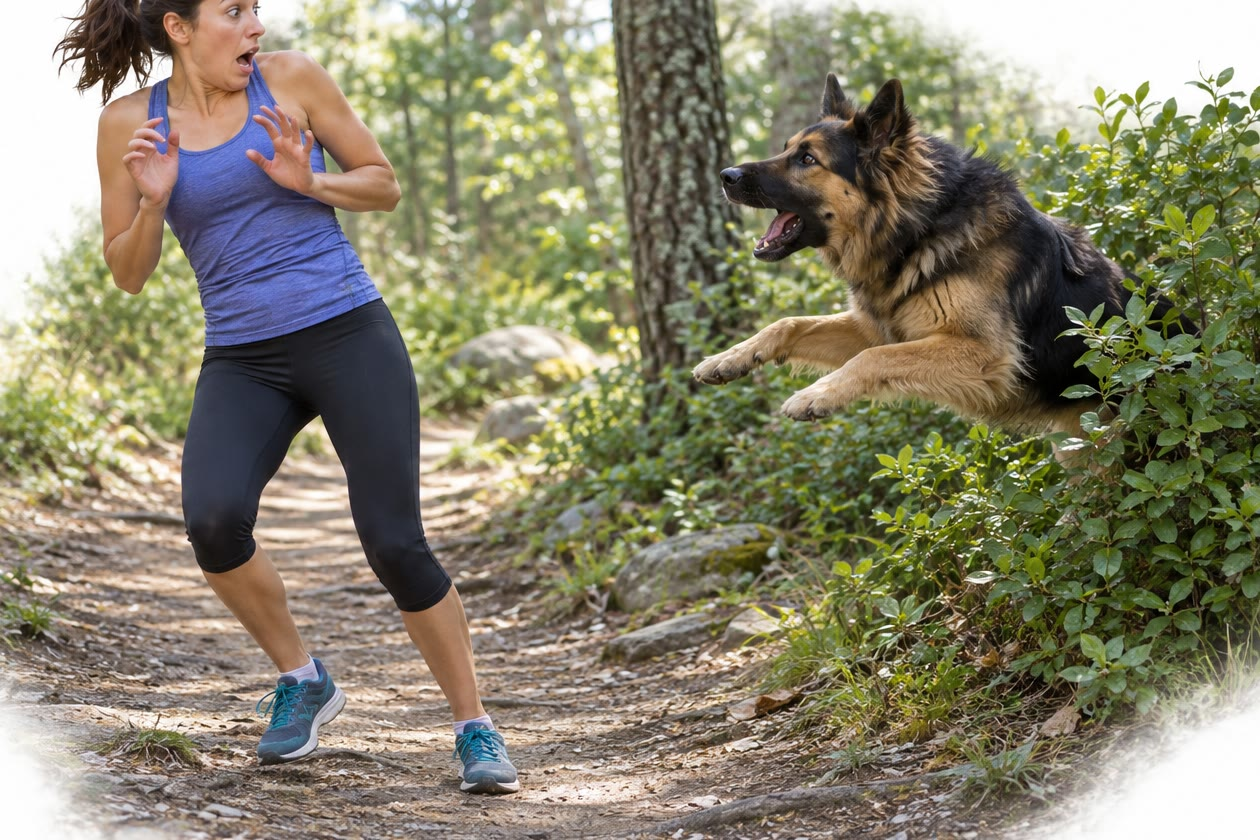
\includegraphics[width=0.6\linewidth]{images/book4/ai/b4-19-adrenaline-runner.jpg}

{\small الشلال في العمل. الفزع يطلق الأدرينالين من
لب الكظر؛ وفي غضون ثوانٍ يتسارع \omterm{def:b2:heart:anatomy}{القلب}، ويصب الكبد
الغلوكوز، وتتسع الطرق الهوائية --- رسول واحد،
ومستقبلات عدة، وتضخيم بمليون ضعف في كل خلية.}
\end{omfigure}

\section{المستقبلات في الداخل}

\begin{proposition}[المستقبلات النووية]\label{prop:b2:cell-signalling:nuclear}
\index{مستقبل نووي}\index{هرمون ستيروئيدي}
تنتشر الستيروئيدات والثيروكسين وحمض الريتينوئيك والفيتامين D عبر
الغشاء وترتبط بمستقبلات في الهيولى أو النواة هي
نفسها \emph{\omterm{prop:b2:cell-differentiation:transcriptional}{عوامل استنساخ}}: فمعقد \omterm{def:b2:cell-signalling:kinds}{الهرمون} والمستقبل
يرتبط بمتواليات معينة من DNA ويشغّل مورّثاته الهدف
أو يطفئها. والاستجابة بطيئة --- من دقائق إلى ساعات لصنع
mRNA والبروتين --- ودائمة: فالكورتيزول يستحث إنزيمات
توليد الغلوكوز ساعات، والإستراديول يبني \omterm{def:b2:reproductive-hormones:cycle}{بطانة الرحم}
على مدى أيام، والتستوستيرون يصنع العضل على مدى أسابيع، والثيروكسين يقرر
معدل استقلاب كل خلية. ولبعض الستيروئيدات أيضًا أفعال سريعة
عبر مستقبلات سطحية، وبعض الطرق السطحية تبلغ
النواة أيضًا (شلال كيناز MAP)، فالتمييز ليس
مطلقًا؛ لكن القاعدة قائمة: إن الرسول الذائب في الدسم
يغير ما \emph{هي} الخلية بتغيير مورّثاتها، بينما الذائب
في الماء يغير ما \emph{تفعله} بتغيير
إنزيماتها.
\end{proposition}

\begin{omfigure}
\begin{tikzpicture}[every node/.style={font=\scriptsize}, >=stealth]
  \foreach \x/\t in {0/{ذائب في الماء: أدرينالين، أنسولين، غلوكاغون}, 7.4/{ذائب في الدسم: كورتيزول، إستراديول، ثيروكسين}} \node[anchor=south, font=\scriptsize\bfseries] at (\x+2.6,3.4) {\t};
  % left: surface receptor
  \fill[omExo!30] (0,2.4) rectangle (5.2,2.8);
  \draw[thick, fill=omDef!40] (1.6,2.1) rectangle (2.3,3.1);
  \fill[omProp] (1.95,3.35) circle (0.1);
  \draw[->, thick] (1.95,2.1) -- (1.95,1.6) node[below, align=center] {رسل ثوانٍ\\وكينازات: إنزيمات\\تُشغَّل في ثوانٍ};
  \node[align=center] at (4.5,1.0) {يغير ما\\تفعله الخلية};
  % right: nuclear receptor
  \begin{scope}[xshift=7.4cm]
    \fill[omExo!30] (0,2.4) rectangle (5.2,2.8);
    \fill[omProp] (1.5,3.35) circle (0.1);
    \draw[->, omProp] (1.5,3.25) -- (1.5,1.9);
    \draw[thick, fill=omThm!20] (1.5,1.5) ellipse (0.72 and 0.3); \node at (1.5,1.5) {مستقبل};
    \draw[thick] (0.6,0.4) -- (4.6,0.4); \draw[thick] (0.6,0.25) -- (4.6,0.25); \node[below] at (2.6,0.2) {DNA: مورّثات هدف تُشغَّل أو تُطفأ، ساعات};
    \draw[->, thick] (1.5,1.2) -- (2.4,0.5);
    \node[align=center] at (4.0,1.4) {يغير ما\\هي الخلية};
  \end{scope}
\end{tikzpicture}

{\small تصميمان. الرسول الذائب في الماء يفعل عند السطح
ويغير فعالية الإنزيمات في غضون ثوانٍ؛ والذائب في الدسم
يدخل، ويرتبط بمستقبل هو \omterm{prop:b2:cell-differentiation:transcriptional}{عامل استنساخ}، فيغير
التعبير المورّثي على مدى ساعات.}
\end{omfigure}

\section{حالة محلولة: الأنسولين والغلوكاغون وقيمة الغلوكوز المرجعية}

\begin{proposition}[هرمونان وقيمة مرجعية]\label{prop:b2:cell-signalling:glucose}
\index{أنسولين}\index{غلوكاغون}\index{غلوكوز الدم}
يُمسك \omterm{prop:b2:cell-signalling:glucose}{غلوكوز الدم} قرب \qty{5}{mmol/L} (\qty{0.9}{g/L})
بهرمونين متضادين من جزر البنكرياس. فبعد وجبة
تستشعر الخلايا $\beta$ ارتفاع الغلوكوز --- إذ
تستقلبه، وتغلق قناة بوتاسيوم إذ يرتفع ATP فيها،
وتستقطب، وتُدخل الكالسيوم، وتطلق \emph{الأنسولين} --- والأنسولين،
عبر مستقبله ذي \omterm{prop:b2:cell-signalling:rtk}{كيناز التيروزين}، يجعل العضل والشحم يلتقطان
الغلوكوز (بنقل الناقلات إلى غشائيهما)، والكبد
يخزنه غليكوجينًا وشحمًا، والأنسجة كلها تكف عن حرق الشحم.
وبين الوجبات يتيح هبوط الغلوكوز للخلايا $\alpha$ أن تطلق
\emph{الغلوكاغون}، الذي يفكك الغليكوجين، عبر \omterm{prop:b2:cell-signalling:gpcr}{AMP الحلقي} في الكبد،
ويصنع غلوكوزًا جديدًا من الحموض الأمينية؛ والأدرينالين يفعل الشيء
نفسه أسرع في الطوارئ، والكورتيزول \omterm{def:b2:cell-signalling:kinds}{وهرمون} النمو على مدى
ساعات. ويُطلق كل \omterm{def:b2:cell-signalling:kinds}{هرمون} بنسبة الانحراف الذي
يصححه: أي تغذية راجعة سالبة بمنفِّذين، واحد لكل
اتجاه، وقيمة مرجعية يُدافع عنها إلى حدود الخُمس. والدماغ،
الذي يحرق \qty{120}{g} من الغلوكوز في اليوم ولا يخزن شيئًا، هو
العضو الذي تحميه الحلقة؛ والسكري من النمط الأول فقد
الخلايا $\beta$، ومساره دون علاج --- غلوكوز عند
\qty{20}{mmol/L}، وشحم يُحرق لغياب الأنسولين، وحمض في الدم
--- هو ما تبدو عليه الحلقة وقد نُزع أحد ذراعيها.
\end{proposition}

\begin{omfigure}
\begin{tikzpicture}
\begin{axis}[
  width=0.82\linewidth, height=5.6cm,
  axis x line=bottom, axis y line=left,
  xmin=0, xmax=6, ymin=0, ymax=1.1,
  xlabel={ساعات بعد وجبة}, ylabel={نسبة إلى الذروة},
  xlabel style={font=\small, at={(axis description cs:0.5,-0.12)}, anchor=north},
  ylabel style={font=\small},
  tick label style={font=\small}, xtick={0,1,2,3,4,5,6}, ytick={0,0.5,1},
  legend style={font=\scriptsize, at={(0.5,-0.28)}, anchor=north, draw=none, legend columns=3},
  clip=false,
]
\addplot[very thick, omDef, domain=0:6, samples=80] {0.55 + 0.45*exp(-((x-0.9)^2)/0.5) - 0.08*exp(-((x-4)^2)/2)};
\addlegendentry{غلوكوز الدم (5 \unit{mmol/L} عند 0.55)}
\addplot[very thick, omThm, domain=0:6, samples=80] {0.15 + 0.85*exp(-((x-1.1)^2)/0.45)};
\addlegendentry{الأنسولين}
\addplot[very thick, omProp, domain=0:6, samples=80] {0.75 - 0.5*exp(-((x-1.2)^2)/0.8) + 0.25*(1-exp(-x/5))*0.6};
\addlegendentry{الغلوكاغون}
\end{axis}
\end{tikzpicture}

{\small الغلوكوز والأنسولين والغلوكاغون بعد وجبة. يرتفع الأنسولين
مع الغلوكوز فيخفضه؛ وإذ يهبط الغلوكوز نحو القيمة
المرجعية، يرتفع الغلوكاغون ليمسكه عندها.}
\end{omfigure}

\begin{example}[سرعة الجملتين ومداهما وكلفتهما]\label{ex:b2:cell-signalling:compare}
يبلغ الأدرينالين في الدم كل خلية في نحو دقيقة
(أي زمن الدوران) ويفعل دقائق؛ أما الدفعة العصبية
فتبلغ هدفها في مليثوان وتفعل مليثوان. \omterm{def:b2:cell-signalling:kinds}{والهرمون}
لا يكلف شيئًا يذكر لكل خلية يبلغها --- نانومول موزع
على الجسم --- لكنه لا يستطيع مخاطبة خلية بعينها؛ أما العصب فيخاطب
خلية واحدة بالضبط لكن عليه بناء سلك إليها وصيانته. والجسم يستعمل
الاثنين: فالأعصاب الودّية في \cref{ch:b2:blood-pressure} تفعل في
\omterm{def:b2:heart:anatomy}{القلب} \omterm{def:b2:blood-circulation:vessels}{والشرينات} في ثانية، ولب الكظر،
وهو نفسه عقدة ودّية معدّلة، يسندها بصب
الجزيء نفسه في الدم للجسم كله. وعند المشبك
يلتقي التصميمان، \omterm{def:b2:cell-signalling:kinds}{فالناقل العصبي} رسول يفعل
في مستقبل بالآليات نفسها --- قناة تنفتح، \omterm{prop:b2:cell-signalling:gpcr}{وبروتين G}
يقلب --- إلا أنه عبر عشرين نانومترًا بدل
متر.
\end{example}

\section{تمارين}

\begin{exercise}[$\star$]\label{exo:b2:cell-signalling:1}
صنّف ما يلي صماويًا أو نظير صماوي أو ذاتيًا أو مشبكيًا، وذائبًا
في الماء أو في الدسم: الأنسولين، والكورتيزول، والأستيل كولين عند
مشبك، والهيستامين عند جرح، والإستراديول، والأدرينالين من
الكظر، وأكسيد النتريك من البطانة.
\end{exercise}

\begin{exercise}[$\star$]\label{exo:b2:cell-signalling:2}
اذكر الخطوات من الأدرينالين عند غشاء الخلية الكبدية إلى الغلوكوز
في الدم، وسمِّ مفتاح الإطفاء عند كل خطوة.
\end{exercise}

\begin{exercise}[$\star$]\label{exo:b2:cell-signalling:3}
قارن بين المستقبلات السطحية والنووية: بم ترتبط، وأين
تقع، وبأي سرعة تفعل، وماذا تغير.
\end{exercise}

\begin{exercise}[$\star$]\label{exo:b2:cell-signalling:4}
ما الرسل الثواني العامة الثلاثة المذكورة في هذا
الفصل، وكيف يُرفع كل منها، وكيف يُزال؟
\end{exercise}

\begin{exercise}[$\star\star$]\label{exo:b2:cell-signalling:5}
لمستقبل $K_d = \qty{2}{nmol/L}$. احسب الإشغال عند
0.2 و2 و20 و\qty{200}{nmol/L}. وخلية تضاعف عدد مستقبلاتها:
فما الذي يتغير، الإشغال أم عدد المستقبلات المشغولة؟
\end{exercise}

\begin{exercise}[$\star\star$]\label{exo:b2:cell-signalling:6}
لشلال مراحل ربوحها 50 و200 و100 و300. احسب
التضخيم الكلي. وإذا كان \omterm{def:b2:cell-signalling:kinds}{الهرمون} عند \qty{1}{nmol/L} وكان
\qty{1}{\%} من المستقبلات ($10^{4}$ في الخلية) مشغولًا، فكم
جزيء ناتج تصنع الخلية في الثانية إذا كان ربح كل مرحلة
في الثانية؟
\end{exercise}

\begin{exercise}[$\star\star$]\label{exo:b2:cell-signalling:7}
يقفل ذيفان الكوليرا \omterm{prop:b2:cell-signalling:gpcr}{بروتين G} المنبّه في حالته المرتبطة
بجزيء GTP في خلايا الأمعاء. فسّر، خطوة خطوة، لماذا يفقد المريض
لترات من السائل في اليوم، ولماذا يدوم الأثر أيامًا بعد
زوال الجراثيم.
\end{exercise}

\begin{exercise}[$\star\star$]\label{exo:b2:cell-signalling:8}
يرتفع الكالسيوم الهيولي من \qty{0.1}{} إلى \qty{1}{\micro
mol/L} في خلية حجمها \qty{2000}{\micro m^3} حين تنفتح قناة. فكم
شاردة كالسيوم دخلت؟ وإذا مررت قناة مفتوحة واحدة $10^{6}$
شاردة في الثانية، فكم استغرقت قناة واحدة، ولماذا تفتح الخلية
كثيرًا منها معًا؟
\end{exercise}

\begin{exercise}[$\star\star$]\label{exo:b2:cell-signalling:9}
يفعل الأنسولين والغلوكاغون كلاهما في الكبد، أحدهما عبر كيناز
تيروزين والآخر عبر \omterm{prop:b2:cell-signalling:gpcr}{AMP الحلقي}. فسّر كيف تدمج الخلية الكبدية
الإشارتين، وماذا يحدث للغليكوجين حين ترتفع الإشارتان معًا،
ولماذا كانت النسبة بينهما أهم من مستوى أي منهما.
\end{exercise}

\begin{exercise}[$\star\star\star$]\label{exo:b2:cell-signalling:10}
يرفع الأدرينالين \omterm{prop:b2:cell-signalling:gpcr}{AMP الحلقي} في خلية كبدية في غضون \qty{5}{s} ويرفع خرج
الغلوكوز في غضون \qty{30}{s}؛ ويرفع الكورتيزول إنزيمات الكبد المولدة
للغلوكوز على مدى \qty{4}{h}. فسّر المقياسين الزمنيين بالانتشار، وبالاستنساخ (\qty{50}{}
نوكليوتيدة في الثانية على مورّثة من \qty{3000}{} نوكليوتيدة)، وبالترجمة
(\qty{5}{} حموض أمينية في الثانية على بروتين من \num{500} بقية)، وبالحاجة
إلى تراكم آلاف من جزيئات الإنزيم.
\end{exercise}

\begin{exercise}[$\star\star\star$]\label{exo:b2:cell-signalling:11}
\omterm{def:b2:genome-diversification:mutation}{طفرة} تجعل مستقبل كيناز تيروزين لعامل نمو
يتثنّى، ومن ثم يشير، دون ربيطته. تنبّأ بسلوك
الخلية، وفسّر لماذا كانت هذه خطوة شائعة في السرطان، وقل
ماذا يفعل دواء يحصر موقع ATP في الكيناز.
\end{exercise}

\begin{exercise}[$\star\star\star$]\label{exo:b2:cell-signalling:12}
«الجملة الصماوية تذيع؛ والجملة العصبية توصل أسلاكًا.»
ناقش التصميمين في السرعة والمدى والنوعية والكلفة، وقل
أين يكون كل منهما لا غنى عنه وأين يستعمل الجسم كليهما
للرسالة نفسها.
\end{exercise}

\section{مسألة: هرمون من الدم إلى المورّثة}

\begin{problem}[{مسألة نهاية الأسبوع --- متابعة الأدرينالين من
غدة الكظر إلى غلوكوز خلية كبدية، مع حساب تركيزه
وإشغاله للمستقبلات وربح شلاله وتوقيته، ثم متابعة الكورتيزول
إلى مورّثة، وتحليل حلقة الغلوكوز، وتنتهي إلى
الإشغال والتضخيم والزمن الذي يستغرقه كل هرمون}]
\label{pb:b2:cell-signalling:1}
المعطيات: يطلق لب الكظر \qty{1}{nmol} من الأدرينالين في
\qty{5}{L} من الدم عند فزع؛ وثابت تفكك الأدرينالين $K_d$ عند مستقبل
الكبد \qty{1}{nmol/L}؛ وتحمل خلية كبدية (\qty{5000}{\micro m^3})
$2\times 10^{4}$ مستقبل. وربوح الشلال في ثانية
التفعيل: مستقبل $\to$ \omterm{prop:b2:cell-signalling:gpcr}{بروتين G} ربحه 20، \omterm{prop:b2:cell-signalling:gpcr}{وبروتين G} $\to$ AMP حلقي 100
(أي دوران السيكلاز في عمر \omterm{prop:b2:cell-signalling:gpcr}{بروتين G} البالغ 3 ثوانٍ)،
وAMP حلقي $\to$ كيناز A ربحه 1 (تكافئيًا)، وكيناز A $\to$ كيناز
الفسفوريلاز 50، $\to$ فسفوريلاز 50، $\to$ غلوكوز 1000. ويحمل الكبد
\qty{100}{g} من الغليكوجين. والكورتيزول: استنساخ عند
\qty{50}{} نوكليوتيدة في الثانية على مورّثة من \qty{4000}{}
نوكليوتيدة، وترجمة عند \qty{5}{} بقايا في الثانية على
إنزيم من \num{600} بقية، و\num{20} ريباسًا لكل mRNA، و\num{100}
mRNA تُصنع في الساعة، وأثر يحتاج $10^{5}$ جزيء إنزيمي.

\medskip
\noindent\textbf{الجزء الأول --- وصول \omterm{def:b2:cell-signalling:kinds}{الهرمون}.}
\begin{enumerate}
  \item احسب تركيز الأدرينالين في \omterm{def:b2:blood-circulation:blood}{البلازما} بعد
        الإطلاق، مهملًا زواله.
  \item احسب \omterm{thm:b2:cell-signalling:occupancy}{إشغال المستقبلات} وعدد المستقبلات المشغولة
        في الخلية الكبدية الواحدة.
  \item يُزال الأدرينالين بعمر نصف قدره \qty{2}{min}. فما
        تركيزه وإشغاله بعد \qty{6}{min}؟
  \item كم يستغرق الأدرينالين ليبلغ الكبد من
        الكظر، إذا كان زمن الدوران نحو دقيقة؟ ولماذا
        يفعل العصب الودّي إلى الكبد أسرع؟
  \item خلية لها $2\times 10^{5}$ مستقبل \omterm{thm:b2:cell-signalling:occupancy}{وثابت التفكك} $K_d$ نفسه:
        فما الذي يتغير؟
  \item لماذا كان $K_d$ مطابقًا للتركيز الدائر ---
        وماذا يفعل مستقبل له $K_d = \qty{1}{\micro mol/L}$
        \omterm{def:b2:cell-signalling:kinds}{بهرمون} نانومولي؟
\end{enumerate}

\medskip
\noindent\textbf{الجزء الثاني --- الشلال.}
\begin{enumerate}[resume]
  \item احسب الربح الكلي من مستقبل مشغول واحد إلى
        جزيئات غلوكوز في الثانية.
  \item احسب جزيئات \omterm{prop:b2:cell-signalling:gpcr}{AMP الحلقي} التي تصنعها الخلية في الثانية
        الأولى، والتركيز الذي تبلغه في حجمها.
  \item احسب خرج الغلوكوز من خلية كبدية واحدة في الثانية عند
        إشغال السؤال 2، وفي الدقيقة.
  \item للكبد $2\times 10^{11}$ خلية. احسب الخرج
        الذي تتنبأ به الربوح، بالغرام في الدقيقة، وقارنه بالقيمة
        \qty{5}{g/min} الملاحظة فعلًا. وما الذي يحد الخرج
        الحقيقي؟
  \item كم تدوم \qty{100}{g} من الغليكوجين بهذا
        المعدل؟ ولماذا لا تنفد في فزع؟
  \item سمِّ مفتاح الإطفاء عند كل مرحلة مضخِّمة وقل أيها
        أسرع فعلًا.
  \item يوجد مثبط للفوسفودي إستيراز (الكافيين). تنبّأ
        بأثره في الشلال وفي خرج الغلوكوز.
\end{enumerate}

\medskip
\noindent\textbf{الجزء الثالث --- الكورتيزول إلى مورّثة.}
\begin{enumerate}[resume]
  \item احسب زمن استنساخ mRNA واحد.
  \item احسب زمن ترجمة جزيء إنزيمي واحد، وعدد
        جزيئات الإنزيم لكل mRNA في الساعة (وكل mRNA
        يعيش ساعة، والريباسات تبدأ واحدًا إثر آخر).
  \item احسب جزيئات الإنزيم المصنوعة في الساعة من
        \num{100} mRNA، وزمن بلوغ $10^{5}$.
  \item أضف زمن دخول الكورتيزول وارتباطه وبلوغه DNA
        (دقائق) وفسّر \qty{4}{h} الملاحظة.
  \item لماذا لا يستعمل الجسم شلالًا كشلال الأدرينالين
        لعمل الكورتيزول، ولا يستعمل آلية الكورتيزول عند
        الفزع؟
  \item يرفع الكورتيزول أيضًا عدد مستقبلات الأدرينالين في
        الخلايا الكبدية. فسّر كيف يستطيع \omterm{def:b2:cell-signalling:kinds}{هرمون} بطيء أن يضخّم
        هرمونًا سريعًا، وماذا يفعل ذلك بمنحني إشغال السريع.
\end{enumerate}

\medskip
\noindent\textbf{الجزء الرابع --- الحلقة.}
\begin{enumerate}[resume]
  \item بعد وجبة يرتفع الغلوكوز من 5 إلى \qty{8}{mmol/L}.
        صف استجابة الخلية $\beta$ من الغلوكوز إلى
        إطلاق الأنسولين، مسميًا الاقتران.
  \item يفعل الأنسولين عبر كيناز تيروزين والغلوكاغون عبر
        \omterm{prop:b2:cell-signalling:gpcr}{AMP الحلقي}. فسّر لماذا تستطيع خلية واحدة أن تطيع الاثنين وكيف
        تُضبط إنزيمات غليكوجين الكبد بنسبتهما.
  \item مريض بلا خلايا $\beta$. تنبّأ بغلوكوزه صائمًا
        وبعد الوجبة، وفسّر لماذا يُحرق الشحم ويظهر
        الحمض.
  \item الأنسولين المحقون بلا تغذية راجعة. فسّر خطر
        عَدْو طويل غير معتاد بجرعة معتادة.
  \item قارن حلقة الغلوكوز \omterm{def:b2:blood-pressure:baroreflex}{بالمنعكس الضغطي} في
        \cref{ch:b2:blood-pressure}: المستشعر والمنفِّذات والربح والسرعة.
  \item اذكر النتيجة: إشغال الأدرينالين بعد الإطلاق،
        وربح الشلال، وخرج الكبد من الغلوكوز، والزمن
        الذي يستغرقه الكورتيزول.
\end{enumerate}
\end{problem}
